Após aplicar os métodos descritos, foram alcançados os seguintes resultados: a criação do site do projeto, utilizando HTML, CSS, JavaScript e NODE.JS, a criação do Diagrama de Classe e Diagrama de Objeto, além do banco de dados físico (MBD).

\textbf{Prototipação do aplicativo no Figma}

A \Cref{fig:landing-page} apresenta a tela de Landing Page do projeto, que permite você se logar ou cadastrar.

\begin{figure}[H]
    \centering
    \caption{Landing Page}
    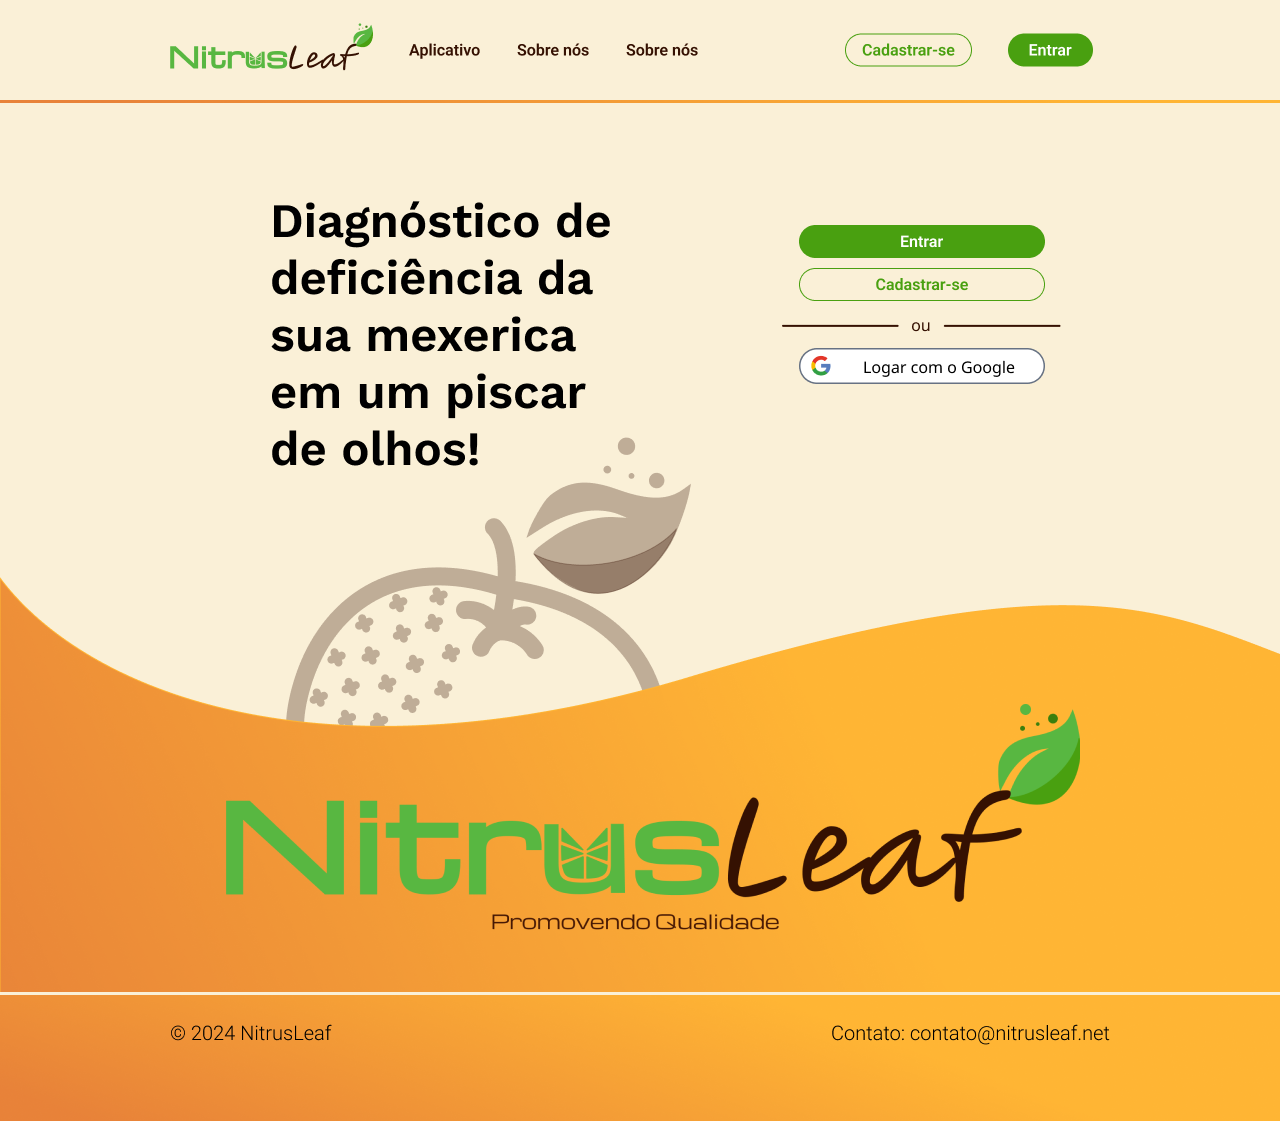
\includegraphics[width=0.7\linewidth]{Illustrations/Landing-Page.png}
    \label{fig:landing-page}
    \SourceOrNote{Autoria Própria (2024)}
\end{figure}

A tela inicial \Cref{fig:tela-inicio} oferece as opções de escanear uma folha com a câmera do celular ou fazer o upload de uma imagem para análise. Abaixo dessas opções, há um gráfico de pizza que mostra a porcentagem das ocorrências totais: amarelo para manganês, laranja-avermelhado para cobre e cinza para “adversos” (casos sem deficiência de cobre ou manganês). No lado direito, um quadro exibe análises recentes, incluindo o número total de plantas analisadas, tratadas e plantadas. No canto esquerdo, um menu permite acesso a outras telas do aplicativo, como histórico, drone e configurações gerais.

\begin{figure}[H]
\centering
\caption{Tela Início}
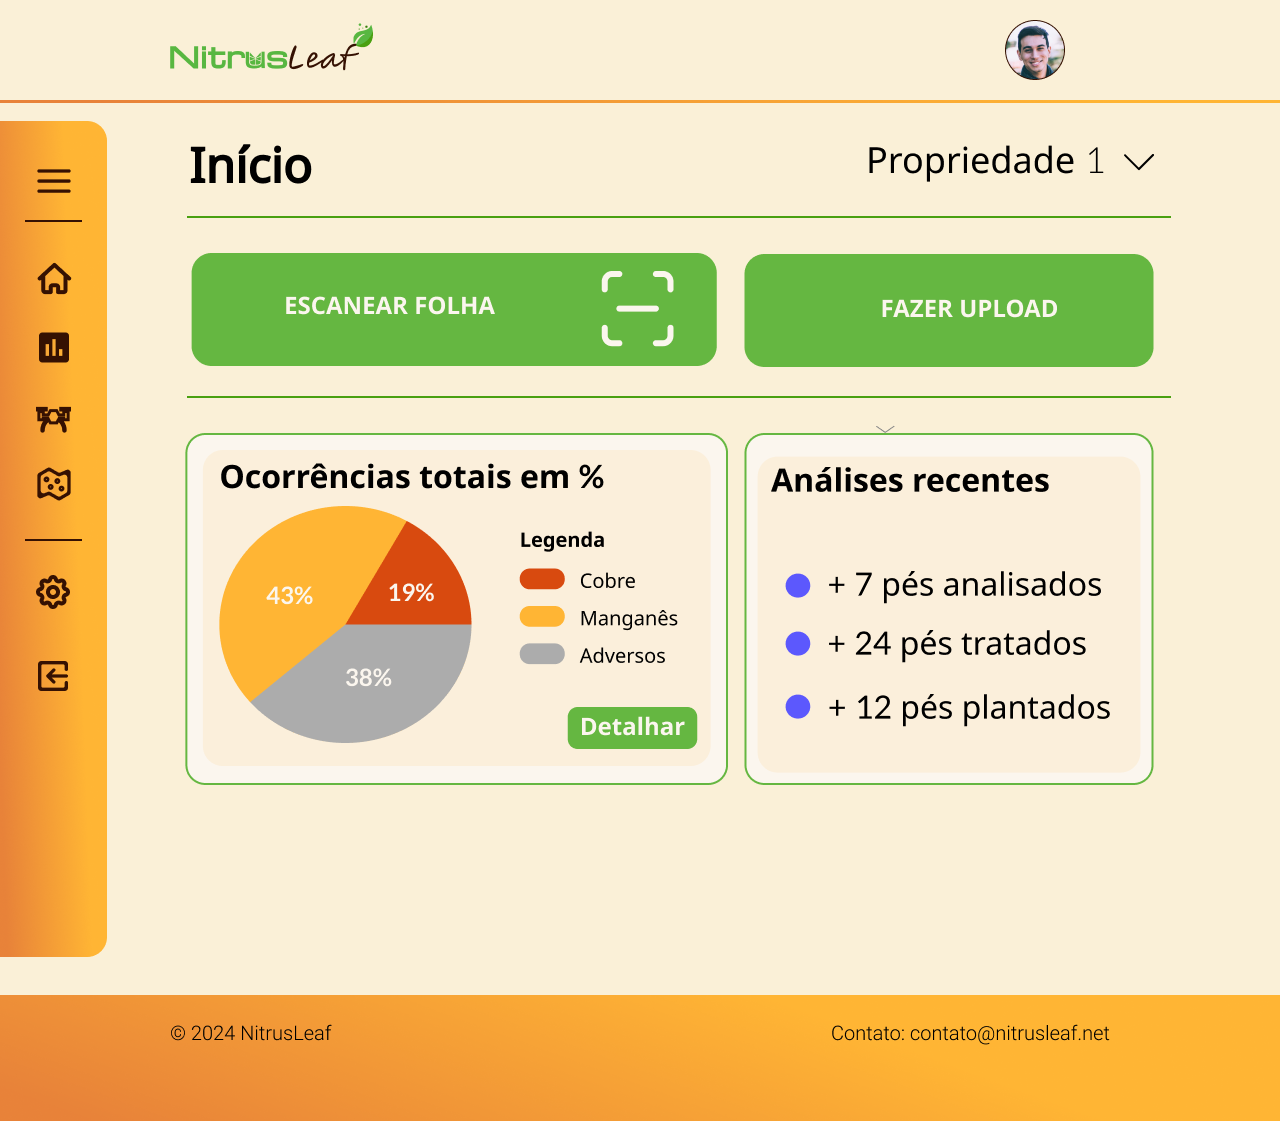
\includegraphics[width=0.7\linewidth]{Illustrations/tela-inicios.png}
\label{fig:tela-inicio}
\SourceOrNote{Autoria Própria (2024)}
\end{figure}

Ao selecionar “escanear folha”, o usuário deverá apontar a câmera para a folha escolhida. Caso opte por fazer o upload de uma imagem, o aplicativo iniciará a análise e, ao concluir, abrirá a tela \Cref{fig:cadastro-diagnóstico} mostrando a probabilidade da deficiência identificada. O usuário deve selecionar a planta analisada, o talhão ao qual pertence e pode adicionar um relatório, se necessário, antes de finalizar.

\begin{figure}[H]
\centering
\caption{Cadastro Diagnóstico}
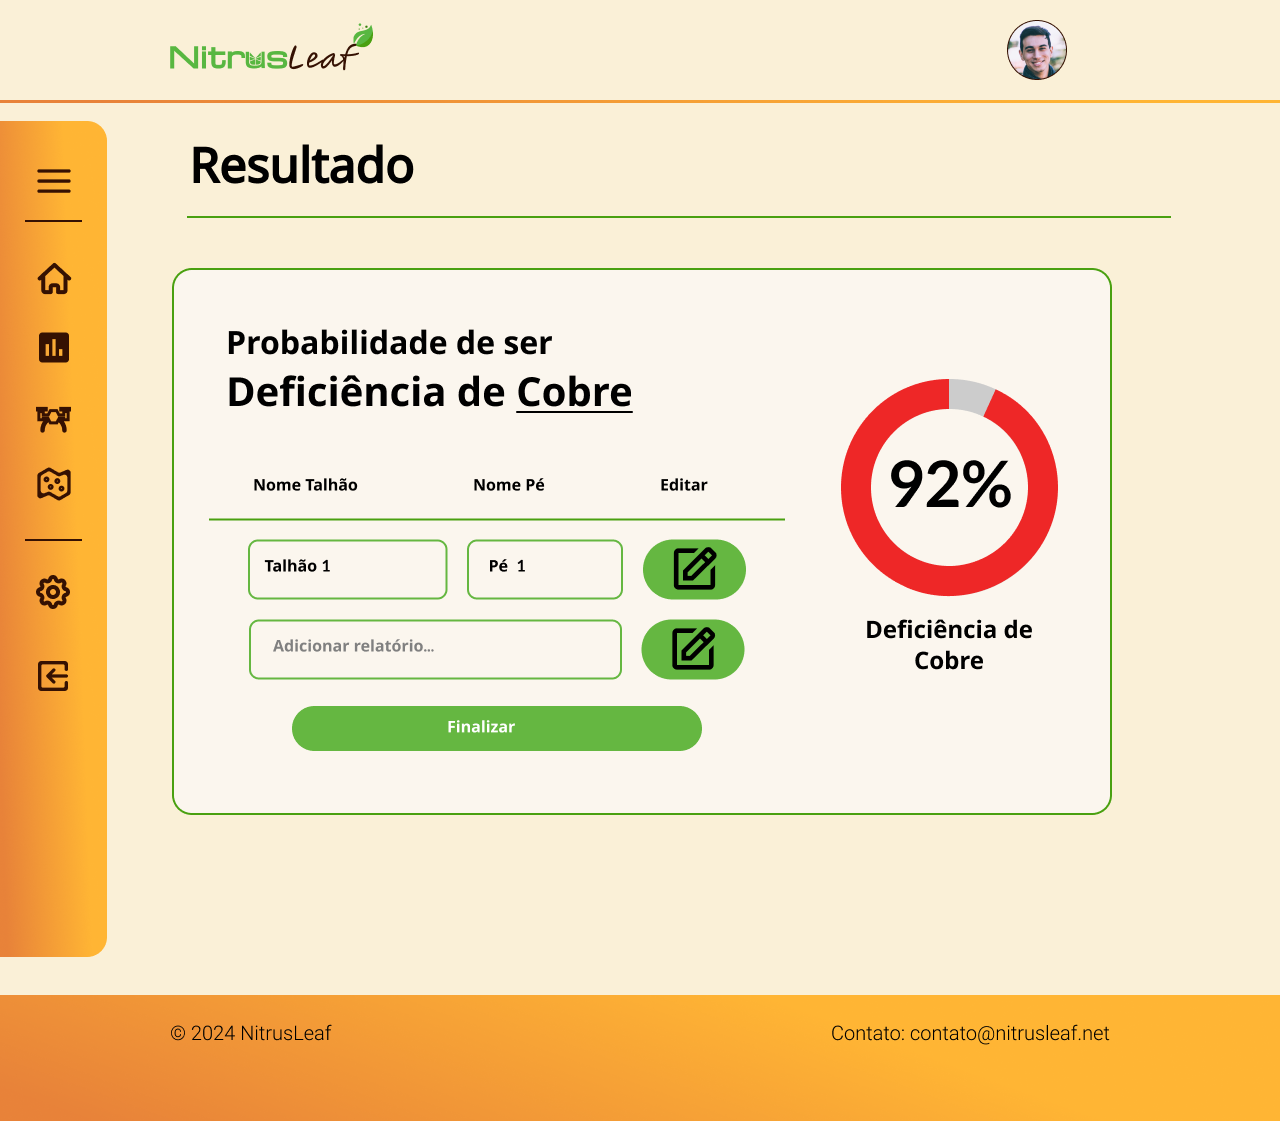
\includegraphics[width=0.8\linewidth]{Illustrations/Tela-Escaneamentos.png}
\label{fig:cadastro-diagnóstico}
\SourceOrNote{Autoria Própria (2024)}
\end{figure}

Para verificar as plantas cadastradas no aplicativo, o usuário acessa a tela de histórico \Cref{fig:tela-relatorios}. Nessa tela, é possível ver a quantidade de plantas cadastradas em cada talhão, selecionar a propriedade sendo verificada, bem como visualizar o número de plantas analisadas até o momento. No lado direito, uma janela exibe o total de talhões e plantas registrados, além do número de plantas analisadas e diagnosticadas.

\begin{figure}[H]
\centering
\caption{Tela Relatórios}
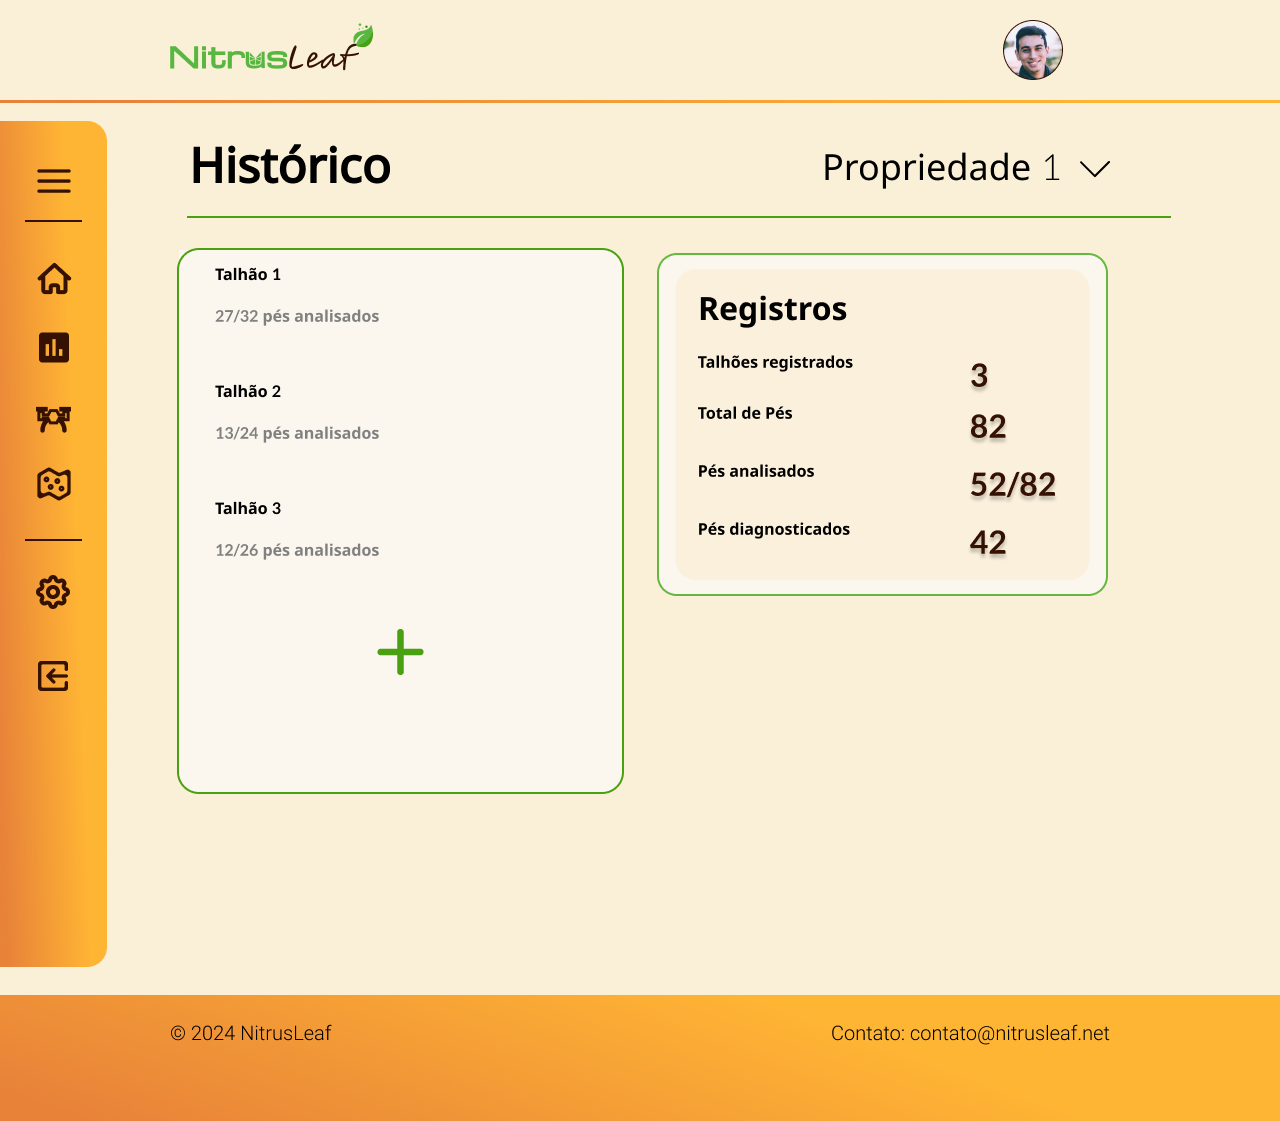
\includegraphics[width=0.7\linewidth]{Illustrations/tela-historico.png}
\label{fig:tela-relatorios}
\SourceOrNote{Autoria Própria (2024)}
\end{figure}

Na tela de mapas \Cref{fig:tela-mapas}, o usuário pode escolher entre diferentes tipos de mapas, como o NDVI, um mapa via satélite que mostra a localização, um mapa com todas as mexericas e um mapa de calor que exibe a concentração de possíveis deficiências.

O NDVI, ou Índice de Estado de Vegetação, é gerado a partir de imagens capturadas por drones e um gráfico de linhas que mostra o nível de NDVI para cada talhão ao longo de 12 meses. Esse índice mede a quantidade de energia refletida e absorvida pelas plantas, fornecendo informações sobre sua saúde com base nessa refletância. A luz visível (400 a 720 nm) é absorvida, enquanto o infravermelho próximo (720 a 1100 nm) é refletido em maior intensidade por plantas saudáveis. Plantas em estresse, desidratadas ou doentes absorvem mais luz infravermelha, o que afeta seu índice NDVI. Esse valor é calculado usando a fórmula: \textit{NDVI} = \((\text{NIR} - \text{VIS}) / (\text{NIR} + \text{VIS})\) \cite{ResultadoNDVIArtigo, ResultadoNDVISite}.

\begin{figure}[H]
\centering
\caption{Mapas}
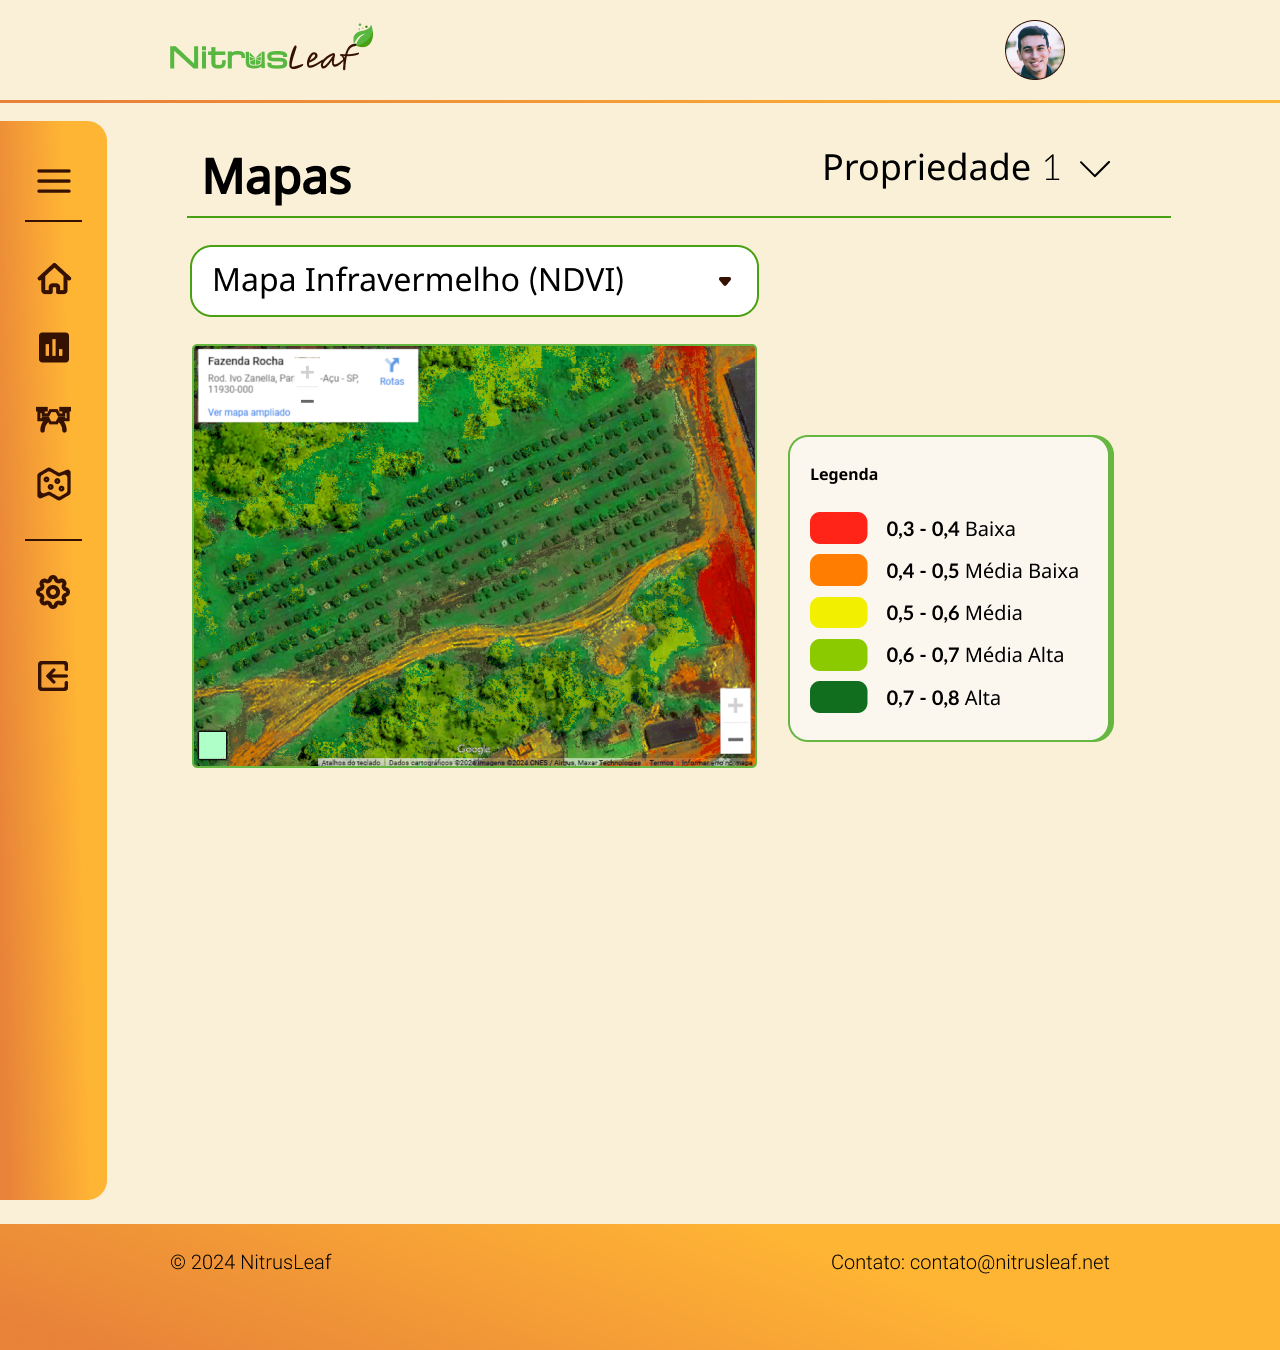
\includegraphics[width=0.7\linewidth]{Illustrations/tela-mapas.png}
\label{fig:tela-mapas}
\SourceOrNote{Autoria Própria (2024)}
\end{figure}

\textbf{Diagrama de Caso de Uso}

O DCU do projeto, ou Diagrama de Caso de Uso, é utilizado para representar as relações entre os atores (usuários do sistema) e as funcionalidades oferecidas pelo projeto. Conforme ilustrado na \Cref{fig:caso-uso}, o diagrama mostra que o proprietário é responsável por cadastrar as mexeriqueiras e os talhões, podendo também se quiser cadastrar drones, consultar gráficos e estatísticas da propriedade. Já o funcionário é encarregado de escanear as folhas, seja utilizando a câmera ou fazendo o upload de imagens. O aplicativo processará essas imagens e fornecerá um diagnóstico baseado nelas. Além disso, o funcionário pode consultar o mapa NDVI gerado pelos drones, acessar o histórico e visualizar estatísticas. Por sua vez, as funções do drone incluem capturar fotos do local e gerar um mapa NDVI.



\begin{figure}[H]
    \centering
    \caption{Diagrama de Caso de Uso}
    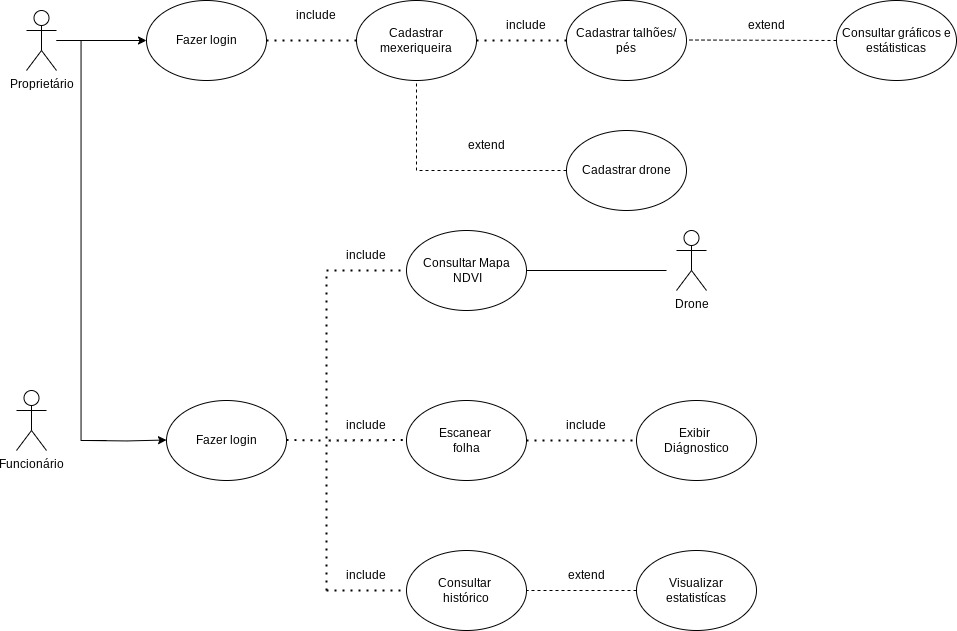
\includegraphics[width=0.7\linewidth]{Illustrations/CasoUso.jpeg}
    \label{fig:caso-uso}
    \SourceOrNote{Autoria Própria (2024)}
    \end{figure}

\textbf{Diagrama de classes}

O diagrama de classes do nosso projeto \Cref{fig:diagrama-classe} começa com a Landing Page, que é a tela inicial exibida caso o usuário não esteja logado. Nessa tela, o usuário pode optar por fazer login ou cadastrar-se. A tela de login permite que o usuário insira seu e-mail ou telefone celular e senha, com a opção de recuperação de senha, caso necessário.

O processo de cadastro envolve a inserção de dados como nome, sobrenome, e-mail, senha, telefone celular, confirmação de senha e endereço. Após essa etapa, o usuário pode continuar o cadastro, especificando o tipo de pessoa (física ou jurídica), CPF ou CNPJ (dependendo do tipo), logradouro, número, bairro e cidade. Em seguida, o sistema permite que o usuário cadastre sua propriedade, incluindo informações como nome, CEP, logradouro, número, bairro e cidade da propriedade. Esse cadastro de propriedade possibilita também a edição de talhões, permitindo ao usuário adicionar o nome do talhão e o nome do pé, com opções de edição ou finalização do cadastro.

Ao escolher escanear uma folha ou fazer o upload de uma imagem, o sistema realiza a análise da imagem e exibe uma tela de resultado que mostra a probabilidade de deficiência identificada ou outras condições. O usuário pode então informar o nome do pé analisado, o talhão ao qual ele pertence e, se necessário, adicionar um relatório à análise. O sistema permite editar o nome do pé, o talhão ou o relatório da análise antes de finalizar o cadastro do resultado.

Há também uma funcionalidade de histórico da propriedade, onde o usuário pode selecionar uma propriedade específica ou alternar para outro talhão, além de adicionar novos talhões. Ao escolher um talhão, o usuário consegue visualizar todos os pés cadastrados nele, podendo buscar um pé pelo nome, selecionar qualquer um dos pés, editar o talhão ou adicionar novos pés. Caso um pé específico seja selecionado, o usuário pode editar o nome, o relatório e, se necessário, excluí-lo do sistema.

Há também a tela Configurações do Usuário, que exibe todos os dados cadastrados, permitindo que o usuário edite suas informações, caso necessário.

\begin{figure}[H]
\centering
\caption{Diagrama de Classe}
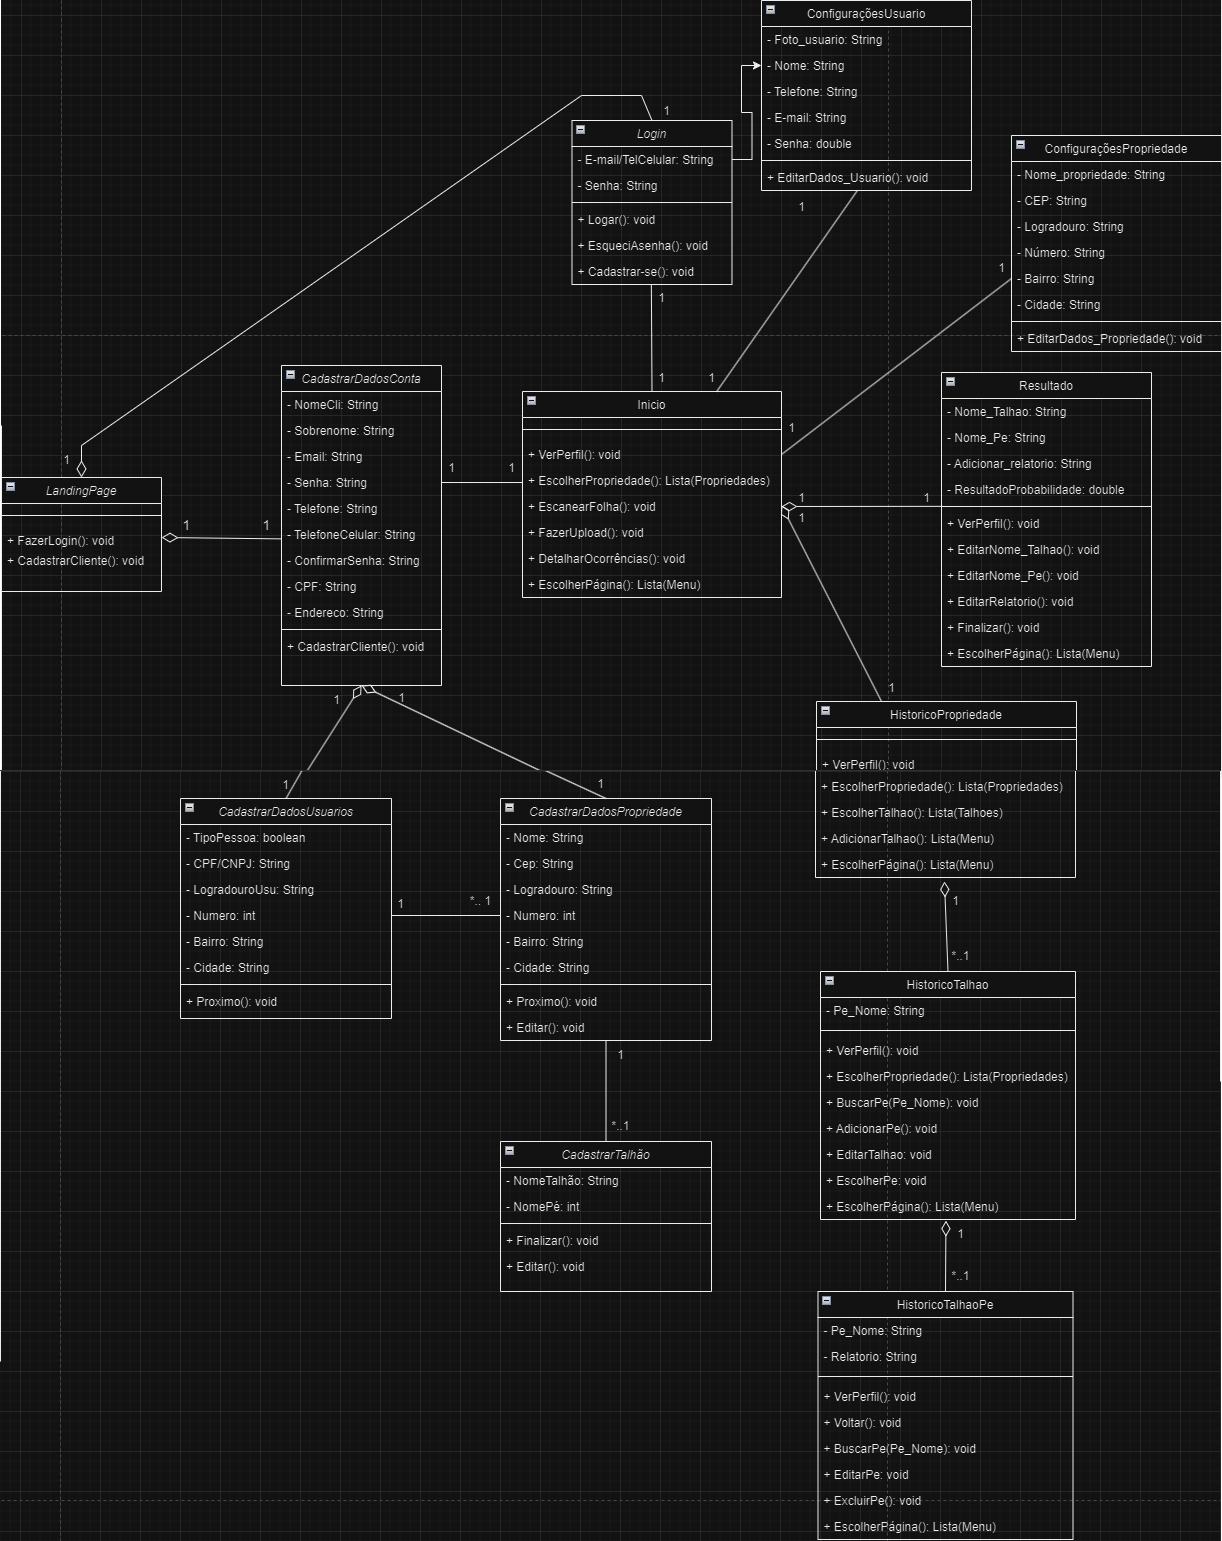
\includegraphics[width=0.7\linewidth]{Illustrations/diagramaClasse.png}
\label{fig:diagrama-classe}
\SourceOrNote{Autoria Própria (2024)}
\end{figure}

\textbf{Diagrama de Objetos}

O diagrama de objetos do nosso projeto \Cref{fig:diagrama-objetos} ilustra o processo de cadastro do usuário, da propriedade e do talhão, destacando as diferenças entre usuários do tipo físico e jurídico.

\begin{figure}[H]
    \centering
    \caption{Diagrama de Objetos}
    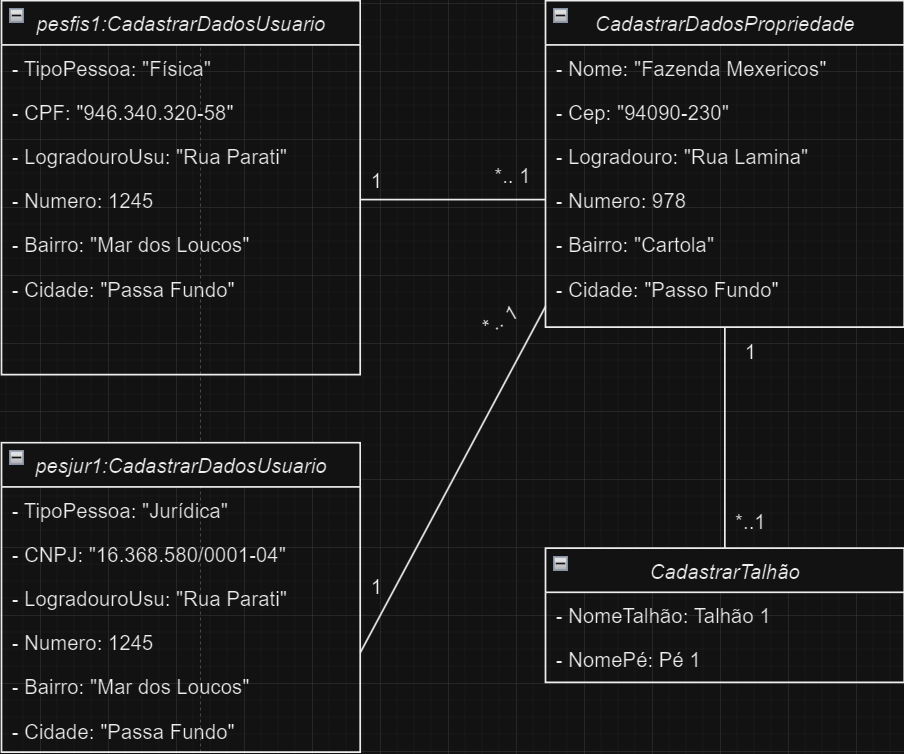
\includegraphics[width=0.7\linewidth]{Illustrations/diagramaObjetos.png}
    \label{fig:diagrama-objetos}
    \SourceOrNote{Autoria Própria (2024)}
    \end{figure}

\textbf{MBD (Modelo de Banco de Dados)}

Primeiramente, é criado o banco de dados, que é então utilizado para gerenciar os dados da aplicação. A seguir, são detalhadas as principais tabelas do banco, e na \Cref{fig:DER} temos o DER do banco de dados físico que será descrito abaixo:

\begin{itemize}
    \item \textbf{Tabela \texttt{usuarios}}: Contém as informações dos usuários. Possui os seguintes campos:
    \begin{itemize}
        \item \texttt{id\_usuario}: Chave primária do tipo \texttt{int}, com \texttt{auto\_increment}.
        \item \texttt{foto\_perfil}: URL da foto de perfil, armazenado em \texttt{varchar}.
        \item \texttt{nome}: Nome do usuário, \texttt{varchar not null}.
        \item \texttt{sobrenome}: Sobrenome do usuário, \texttt{varchar not null}.
        \item \texttt{email}: E-mail do usuário, \texttt{varchar not null}.
        \item \texttt{senha}: Senha do usuário, \texttt{varchar not null}.
        \item \texttt{telefone}: Telefone, \texttt{varchar not null}.
        \item \texttt{celular}: Celular, \texttt{varchar not null}.
        \item \texttt{tipo\_pessoa}: Tipo de pessoa, \texttt{enum} com valores “fisica” ou “juridica”, \texttt{not null}.
        \item \texttt{cpf}: CPF, armazenado em \texttt{varchar}, obrigatório para pessoas físicas.
        \item \texttt{cnpj}: CNPJ, \texttt{varchar}, obrigatório para pessoas jurídicas.
        \item \texttt{nome\_fantasia}: Nome fantasia da empresa, \texttt{varchar}.
        \item \texttt{logradouro}, \texttt{numero}, \texttt{bairro}, \texttt{cidade}: Campos de endereço em \texttt{varchar}.
        \item \texttt{cep}: CEP, \texttt{varchar}.
    \end{itemize}

    \item \textbf{Tabela \texttt{propriedades}}: Armazena as informações das propriedades dos usuários.
    \begin{itemize}
        \item \texttt{id\_propriedade}: Chave primária do tipo \texttt{int}, com \texttt{auto\_increment}.
        \item \texttt{id\_usuario}: Chave estrangeira que referencia o usuário proprietário, tipo \texttt{int}.
        \item \texttt{nome\_propriedade}, \texttt{logradouro\_propriedade}, \texttt{numero\_propriedade}, \texttt{bairro\_propriedade}, \texttt{cep\_propriedade}, \texttt{cidade\_propriedade}: Campos de identificação e localização, todos do tipo \texttt{varchar}.
        \item \texttt{talhoes\_registrados}: Total de talhões registrados, \texttt{int} com valor padrão \texttt{0}.
        \item \texttt{total\_pes}: Total de pés cadastrados na propriedade, \texttt{int} com valor padrão \texttt{0}.
        \item \texttt{pes\_analisados}: Total de pés analisados, \texttt{int} com valor padrão \texttt{0}.
        \item \texttt{pes\_diagnosticados}: Número de pés diagnosticados, \texttt{int} com valor padrão \texttt{0}.
    \end{itemize}
    A chave estrangeira \texttt{id\_usuario} referencia a tabela \texttt{usuarios}.

    \item \textbf{Tabela \texttt{talhoes}}: Armazena as informações dos talhões.
    \begin{itemize}
        \item \texttt{id\_talhao}: Chave primária do tipo \texttt{int}, com \texttt{auto\_increment}.
        \item \texttt{id\_propriedade}: Chave estrangeira que referencia a propriedade à qual o talhão pertence.
        \item \texttt{nome}: Nome do talhão, \texttt{varchar not null}.
        \item \texttt{especie\_fruta}: Espécie da fruta, \texttt{varchar not null}.
    \end{itemize}
    A chave estrangeira \texttt{id\_propriedade} referencia a tabela \texttt{propriedades}.

    \item \textbf{Tabela \texttt{pes}}: Representa cada pé plantado no talhão.
    \begin{itemize}
        \item \texttt{id\_pe}: Chave primária do tipo \texttt{int}, com \texttt{auto\_increment}.
        \item \texttt{id\_talhao}: Chave estrangeira que referencia o talhão ao qual o pé pertence.
        \item \texttt{nome}: Nome do pé, \texttt{varchar not null}.
        \item \texttt{situacao}: Situação do pé, \texttt{enum} com valores “tratado”, “nao tratado” e “sem informacoes”, \texttt{not null}.
    \end{itemize}
    A chave estrangeira \texttt{id\_talhao} referencia a tabela \texttt{talhoes}.

    \item \textbf{Tabela \texttt{fotos}}: Armazena as fotos tiradas de cada pé para análise.
    \begin{itemize}
        \item \texttt{id\_foto}: Chave primária do tipo \texttt{int}, com \texttt{auto\_increment}.
        \item \texttt{id\_pe}: Chave estrangeira que referencia o pé da qual a foto foi tirada.
        \item \texttt{id\_talhao}: Chave estrangeira que referencia o talhão ao qual o pé pertence.
        \item \texttt{url}: URL da foto, \texttt{varchar not null}.
        \item \texttt{data\_tirado}: Data em que a foto foi tirada, \texttt{date}.
        \item \texttt{resultado\_analise}: Resultado da análise da imagem, \texttt{varchar}.
    \end{itemize}
    As chaves estrangeiras \texttt{id\_pe} e \texttt{id\_talhao} referenciam, respectivamente, as tabelas \texttt{pes} e \texttt{talhoes}.

    \item \textbf{Tabela \texttt{relatorios}}: Armazena relatórios de diagnóstico para cada pé.
    \begin{itemize}
        \item \texttt{id\_relatorio}: Chave primária do tipo \texttt{int}, com \texttt{auto\_increment}.
        \item \texttt{id\_pe}: Chave estrangeira que referencia o pé analisado.
        \item \texttt{id\_foto}: Chave estrangeira que referencia a foto utilizada no relatório.
        \item \texttt{deficiencia\_cobre}: Verifica deficiência de cobre, \texttt{boolean} com valor padrão \texttt{false}.
        \item \texttt{deficiencia\_manganes}: Verifica deficiência de manganês, \texttt{boolean} com valor padrão \texttt{false}.
        \item \texttt{outros}: Indica se o resultado foi adverso, \texttt{boolean} com valor padrão \texttt{false}.
        \item \texttt{nao\_analisado}: Indica se a planta ainda não foi analisada, \texttt{boolean} com valor padrão \texttt{true}.
        \item \texttt{observacoes}: Observações adicionais do usuário, \texttt{varchar}.
        \item \texttt{data\_analise}: Data em que a análise foi realizada, \texttt{date not null}.
    \end{itemize}
    As chaves estrangeiras \texttt{id\_pe} e \texttt{id\_foto} referenciam, respectivamente, as tabelas \texttt{pes} e \texttt{fotos}.
\end{itemize} 
\textbf{DER do Banco de dados}
\begin{figure}[H]
\centering
\caption{DER}
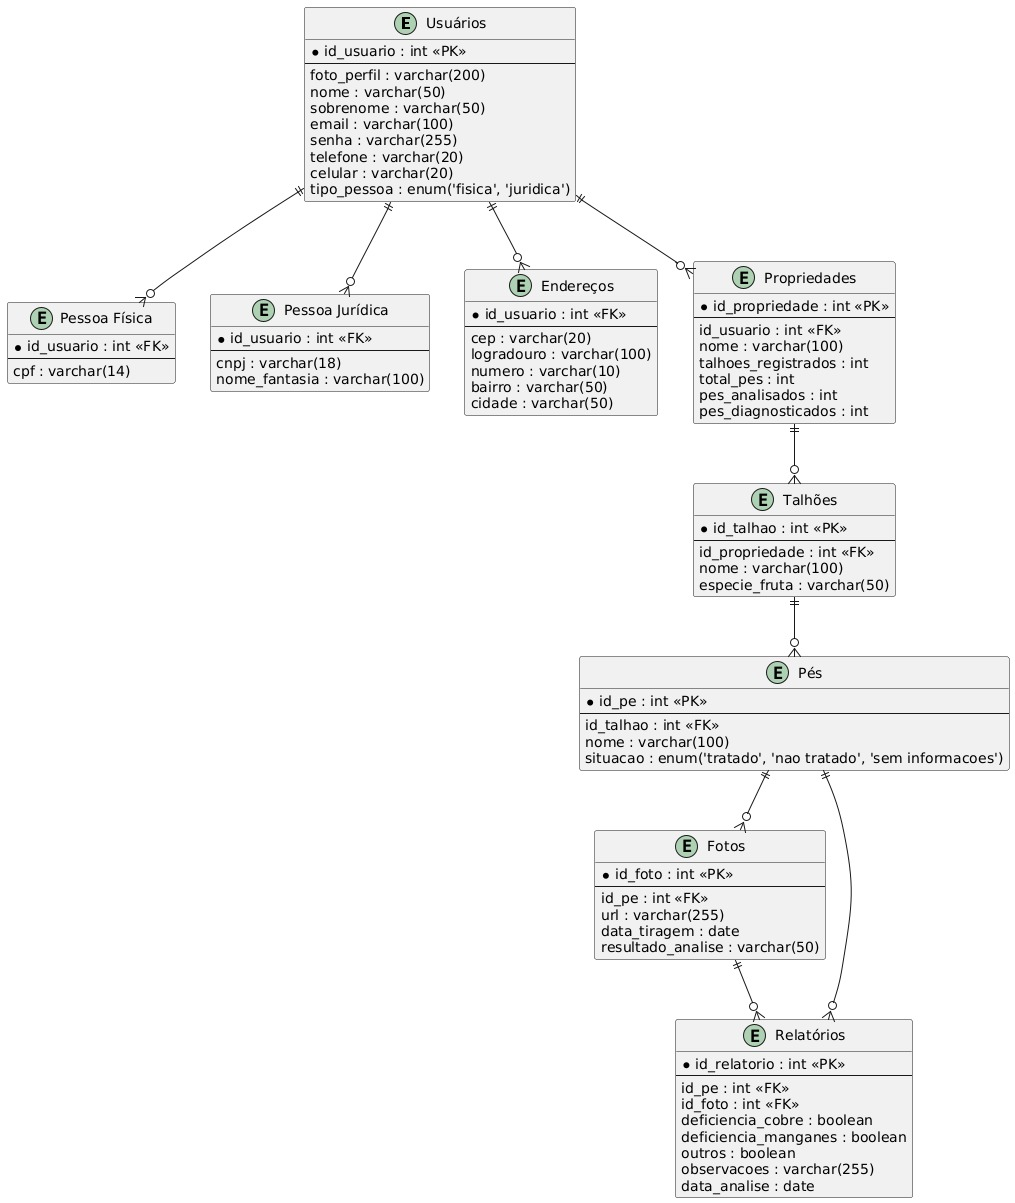
\includegraphics[width=0.7\linewidth]{Illustrations/DER_BD.jpeg}
\label{fig:DER}
\SourceOrNote{Autoria Própria (2024)}
\end{figure}

\textbf{Algoritmo de ordenação}

O algoritmo de ordenação escolhido foi o Quick Sort, que foi selecionado por ser altamente adequado para grandes volumes de dados, o que pode ser uma realidade em cenários como o gerenciamento de uma plantação, onde existem muitos pés em um talhão. O Quick Sort é eficiente em termos de desempenho, com uma complexidade média de O(n log n), o que o torna ideal para lidar com grandes quantidades de informações. Além disso, ele oferece um excelente equilíbrio entre desempenho e simplicidade de implementação, facilitando a sua adoção no código. Outro ponto relevante é que o Quick Sort é um algoritmo in-place, ou seja, ele ordena os dados sem a necessidade de alocar espaço extra significativo para armazenar cópias dos dados, o que o torna mais eficiente em termos de uso de memória. No contexto do código, o Quick Sort foi utilizado para ordenar os registros pela data de criação, priorizando os dados mais recentes (do mais novo para o mais velho), o que é crucial para garantir que as informações mais atuais sejam processadas e apresentadas com maior relevância.

Dentro do Quick Sort, o pivô é um elemento selecionado do array que será usado para dividir os dados em duas partes. O objetivo do pivô é organizar os dados ao seu redor, de forma que todos os elementos menores que o pivô fiquem à esquerda dele e todos os elementos maiores fiquem à direita. Este processo de divisão e conquista continua de forma recursiva até que o array esteja totalmente ordenado. O pivô, portanto, desempenha um papel fundamental no funcionamento eficiente do algoritmo, garantindo que a ordenação seja realizada de maneira progressiva.

Logo abaixo do pseudocódigo do algoritmo, está a tela \Cref{fig:tela-alg}, que mostra a implementação do algoritmo em prática.

\begin{algorithm}
    \caption{Algoritmo QuickSort para ordenar os pés de um talhão pela data}
    \begin{algorithmic}[1]
    \Function{QuickSort}{pes, data\_criacao}
        \If{tamanho(pes) $\leq$ 1}
            \State \Return pes
        \EndIf
    
        \State pivô $\gets$ pes[tamanho(pes) - 1]
        \State esquerda $\gets$ []
        \State direita $\gets$ []
    
        \State dataPivô $\gets$ \Call{toDate}{pivô.data\_criacao}
    
        \For{$i \gets 0$ \textbf{até} tamanho(pes) - 2}
            \State dataAtual $\gets$ \Call{toDate}{pes[i].data\_criacao}
            \If{dataAtual $>$ dataPivô}
                \State esquerda.add(pes[i])
            \Else
                \State direita.add(pes[i])
            \EndIf
        \EndFor
    
        \State \Return \Call{QuickSort}{esquerda, data\_criacao} + [pivô] + \Call{QuickSort}{direita, data\_criacao}
    \EndFunction
    \end{algorithmic}
\end{algorithm}


Caso Base:
\[
\text{QuickSort}(pes) = pes \quad \text{se} \quad \text{tamanho}(pes) \leq 1
\]

Caso Geral:
\[
\text{QuickSort}(pes) = \text{QuickSort}(\text{esquerda}) + \{ \text{pivô} \} + \text{QuickSort}(\text{direita})
\]
onde:

- \text{esquerda} contém os elementos menores que o pivô.
- \text{direita} contém os elementos maiores ou iguais ao pivô.
- A recursão é aplicada nas sublistas \text{esquerda} e \text{direita}.
   
\begin{figure}[H]
\centering
\caption{Tela histórico de pés}
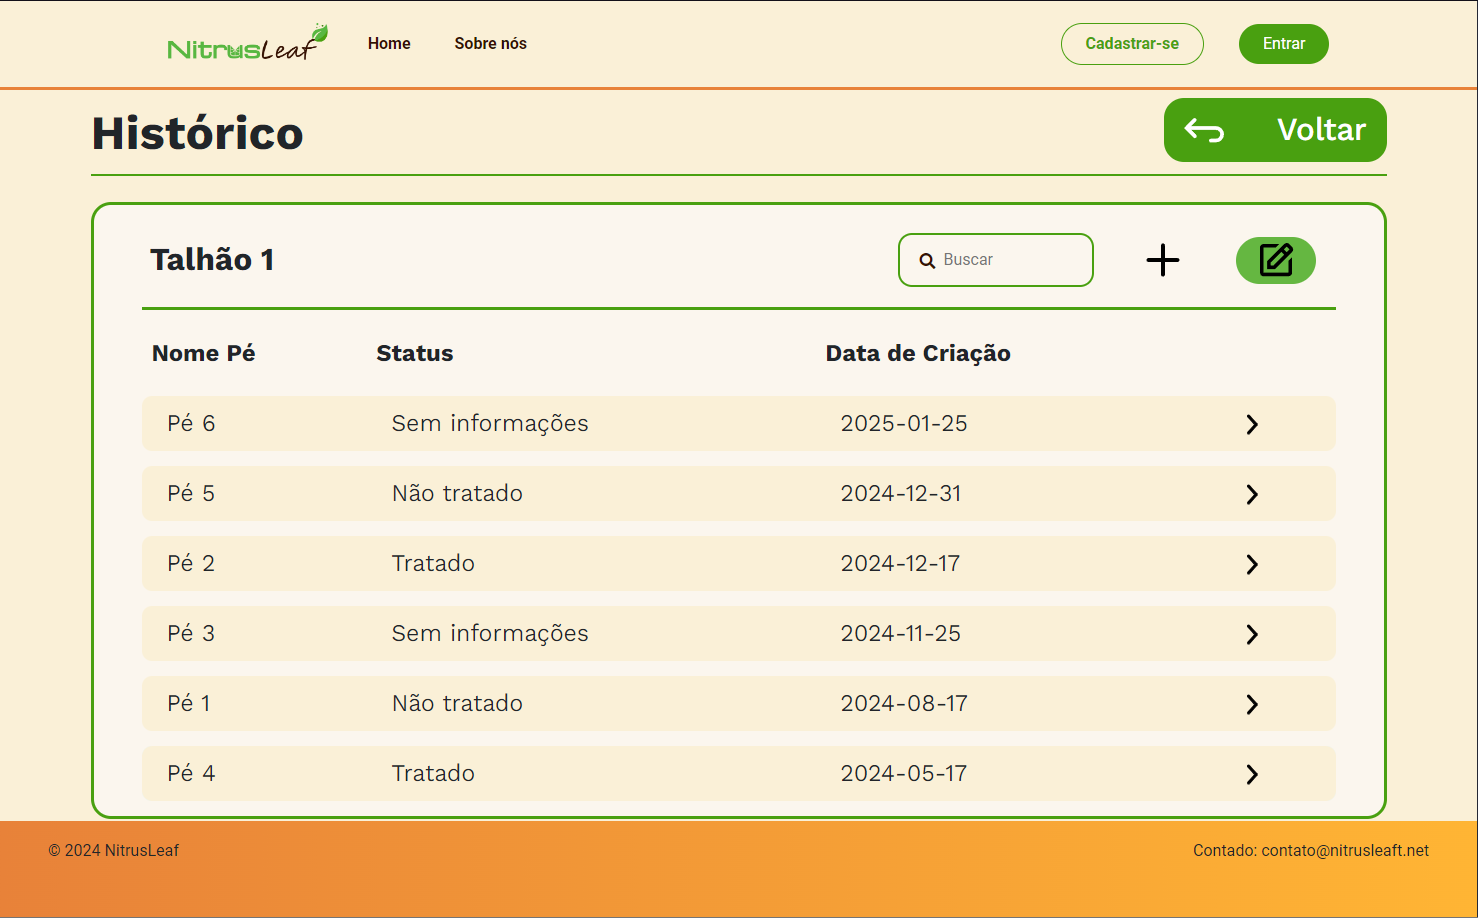
\includegraphics[width=0.7\linewidth]{Illustrations/tela_hist.png}
\SourceOrNote{Autoria Própria (2024)}
\label{fig:tela-alg}
\end{figure}

\textbf{Modelo de negócios Canvas}
    
    O modelo de negócios Canvas do projeto NitrusLeaf \Cref{fig:canvaspi} tem como principal objetivo delinear os elementos cruciais para o sucesso do nosso empreendimento. Esse modelo abrange várias áreas essenciais, incluindo nossos parceiros, proposta de valor, relacionamento com o cliente, recursos e atividades chave, canais, estrutura de custos e fontes de renda.
    
    Parceiros Chave
    
    Nosso foco principal em parceiros chave são os locais e entidades envolvidas no setor agrícola, especialmente aqueles interessados em inovação tecnológica. Esses parceiros incluem cooperativas agrícolas, universidades, centros de pesquisa, empresas de tecnologia agrícola, secretarias de agricultura dos municípios do Vale do Ribeira e associações de fazendeiros. A colaboração com esses parceiros é fundamental para ampliar o alcance do projeto e assegurar suporte técnico e científico.
    
    Proposta de Valor
    
    A proposta de valor do NitrusLeaf gira em torno da capacidade de identificar deficiências nutricionais nas plantas, especificamente a falta de manganês e cobre nas folhas de mexerica, de maneira eficiente e em tempo real. Além disso, o projeto visa manter um padrão elevado de qualidade dos frutos, ajudando os agricultores a otimizar a saúde das plantas e a produtividade.
    
    Relacionamento com o Cliente
    
    O relacionamento com o cliente é focado em oferecer um suporte abrangente. Isso inclui suporte técnico para a utilização do aplicativo via WhatsApp e feedback do cliente pelo app, além de canais de comunicação para feedback e resolução de dúvidas. Nosso objetivo é garantir que os clientes se sintam apoiados e possam maximizar os benefícios do nosso sistema.
    
    Recursos Chave
    
    Os recursos chave para o desenvolvimento e operação do NitrusLeaf incluem infraestrutura tecnológica (servidores, drones, câmeras de alta resolução), conhecimento técnico em agronomia e TI, uma equipe de suporte dedicada, programadores, instaladores do sistema físico, funcionários para suporte online e host para hospedar o site. Esses recursos são essenciais para o funcionamento eficaz do sistema.
    
    Atividades Chave
    
    As atividades chave do projeto incluem o desenvolvimento contínuo do software, a calibração dos algoritmos de IA para identificar deficiências nutricionais, a manutenção dos drones e outros equipamentos, e a realização de testes de campo para validar os diagnósticos fornecidos pelo sistema.
    
    Canais
    
    Os canais através dos quais promovemos e oferecemos nossos serviços incluem nosso website, redes sociais, feiras agrícolas, eventos de tecnologia, newsletters, parcerias com distribuidores agrícolas e anúncios pelas secretarias de agricultura dos municípios do Vale do Ribeira.
    
    Estrutura de Custos
    
    A estrutura de custos engloba despesas com desenvolvimento e manutenção do software, compra e manutenção de equipamentos (drones e câmeras), marketing e promoção, salários da equipe, custos operacionais gerais como servidores e infraestrutura de TI, manutenção dos itens que realizam o monitoramento das mexericas, compra dos produtos necessários para o monitoramento, host para hospedar as informações, aluguel do sistema e itens necessários, e mão de obra para instalação e manutenção.
    
    Fontes de Renda
    
    A principal fonte de renda do NitrusLeaf provém da venda de assinaturas para o uso do aplicativo, serviços de análise de solo e plantas, consultoria técnica, parcerias com empresas e aluguel do sistema.
    
    Em resumo, o modelo de negócios Canvas do NitrusLeaf oferece uma visão abrangente de como estruturamos nosso projeto para atingir nossos objetivos e atender às necessidades dos nossos clientes. Nossa abordagem integrada garante que todos os aspectos do negócio estejam alinhados para promover a saúde e produtividade das plantações de nossos usuários.